\chapter{L'offre \og plateformes d'intégration continue \fg}
\label{section:pic}

\paragraph{}
Quand on sait que 70\% des projets informatiques ne respectent pas le planning initial ou se transforment en échecs~\cite{echec}, on cherche par tous les moyens à réduire les facteurs responsables.
Le manque de qualité logicielle et de suivi de projet en font évidemment parti.
Alors que ces domaines étaient encore un marché de niche il y a quelques temps de cela, aujourd'hui, de plus en plus de clients et de DSI\footnote{Directions de Services Informatiques} commencent à s'en préoccuper et à remettre en cause les méthodes classiques de gestion de projets informatiques.
C'est aussi l'occasion de tenter de pérenniser les développements qui au fil de leurs évolutions perdent paradoxalement en maintenabilité.

\paragraph{}
La qualité logicielle et le suivi de projets informatiques deviennent donc un véritable enjeu actuel.
Les entreprises doivent alors se doter de nouveaux process et de nouveaux outils. 
Elles peuvent les acquérir en faisant notamment appel à des prestations de conseil dans le domaine, qui font entre autres intervenir des notions de gestion de projet et de bonnes pratiques en terme de génie logiciel.
Au-delà de ça, les nouveaux outils doivent être mis en place et intégrés aux infrastructures systèmes existantes.

\paragraph{}
C'est ainsi que la \abusys{} de \asmile, sous l'impulsion de \agulet, s'est positionnée sur ce marché.
Une offre open source a été construite pour répondre au besoin de A à Z, de l'installation des outils au conseil sur leur utilisation, en passant par leur configuration personnalisée.


\section{Intérêt des méthodes agiles}

\paragraph{}
Les méthodes agiles sont très répandues dans les communautés du logiciel libre.
Les programmes y sont souvent développés en en suivant les principes.
Raison de plus pour que \asmile{}, leader sur le marché de l'open source, fasse la promotion de l'agilité après des entreprises.


\paragraph{}
Les méthodes agiles partent du constat que les spécifications initiales du client sont souvent \og volatiles \fg, dans le sens où elles évoluent relativement vite dans le temps et qu'elles souffrent régulièrement d'imprécision.
Les méthodes lourdes classique de développement impliquant spécifications, réalisation puis recette par le client se révèlent donc inadaptées.
Au contraire, il faut privilégier des cycles de développement courts qui apportent la flexibilité nécessaire pour pouvoir corriger rapidement à coût moindre les éventuelles erreurs de spécification ou de conception.

L'organisation du développement épouse alors deux aspects :

\begin{itemize}
	\item le côté itératif, car le logiciel est créé sur plusieurs cycles d'une durée relativement courte ;
	\item l'aspect incrémental, car chaque nouveau cycle améliore les fonctionnalités du précédent.
\end{itemize}


\paragraph{}
En outre, le Manifeste Agile~\cite{agile}, considéré comme l'acte généralisateur des méthodes agiles, invite à adopter un certain nombre de valeurs :

\begin{itemize}
	\item il faut privilégier les personnes et les interactions plutôt que de suivre aveuglément des procédures et d'être dirigé par ses outils ;
	\item la création régulière de jalons fonctionnels est une priorité pour garder constamment à l'idée ce qu'est et ce que va être le produit final ;
	\item la clé est la collaboration étroite avec le client, alors que l'on a traditionnellement tendance à respecter un contrat et à suivre des spécifications initiales ;
	\item le client et le prestataire réalisateur doivent tous deux être flexible et accepter le changement.
\end{itemize}


\paragraph{}
Les méthodes agiles sont parfois difficiles à mettre en place car elles sont souvent en rupture avec les processus existants de l'entreprise.
De plus, la flexibilité requise peut être confondue avec un défaut d'organisation, ce qui amène inévitablement à des résultats catastrophiques.
Au contraire, de bons outils adaptés sont nécessaires pour effectuer un vrai suivi du projet.
Ils doivent permettre de tracer de façon transparente les changements et d'améliorer la communication entre les différents acteurs du projet.



\section{La gestion de projet agile}

\paragraph{}
L'outil de gestion de projet est évidemment un point central de l'offre.
Il permet de suivre en détail le projet, de planifier les différentes étapes de l'évolution du logiciel, de suivre les changements dans le code et de rapporter des bugs.
Certains outils permettent même d'accéder à des fonctionnalités plus poussées comme la rédaction de documentation relative au projet, la gestion du temps passé sur chaque tâche, une gestion documentaire ou encore la planification de l'allocation de ressources.

\paragraph{}
La clé de l'outil de gestion de projet est le système de gestion des tâches, plus souvent dénommé \etranger{bugtracker}.

Chaque tâche est représentée par une entrée dans le système, appelée \textit{ticket}, \textit{demande} ou \textit{rapport de bug} selon les outils.
Elle dispose d'un titre et d'une description qui permettent de savoir en quoi elle consiste.
Elle possède également un statut dont le but est de préciser son état d'avancement : de façon minimaliste, le statut peut prendre les valeurs \og non réalisé \fg, \og en cours \fg{} et \og terminé \fg{} par exemple.
De plus, une tâche peut être attribuée à un utilisateur du système qui sera considéré comme la personne en charge de sa réalisation.
Une date d'échéance peut aussi être définie.
En outre, il existe souvent une fonctionnalité de commentaires qui permet aux utilisateurs de partager leur avis ou leur avancement.

Ainsi, le système de gestion des tâches est véritablement l'élément permet de suivre l'avancement du projet.
La granularité est plus ou moins fine en fonction du découpage en tâches qui est pratiqué.

\paragraph{}
Par ailleurs, il est possible d'utiliser un outil de gestion de projet agile pour suivre des tâches qui n'ont rien à voir avec celles d'un projet informatique.
Grâce à un système de gestion des tâches suffisamment généraliste et/ou personnalisé, il est possible de planifier des activités allant de l'organisation d'une réunion, le changement d'une ampoule en passant par la rédaction d'un rapport.

C'est avec ce type de problématique que les prestations de conseil deviennent deviennent incontournables.
Une bonne expérience et de bonnes connaissances sur les possibilités de l'outil permettent de segmenter efficacement les besoins de l'entreprise en entités et projets.
En effet, cela doit permettre aux utilisateurs finaux de mettre à profit le système de manière claire et efficace.

\begin{figure}
	\centering
	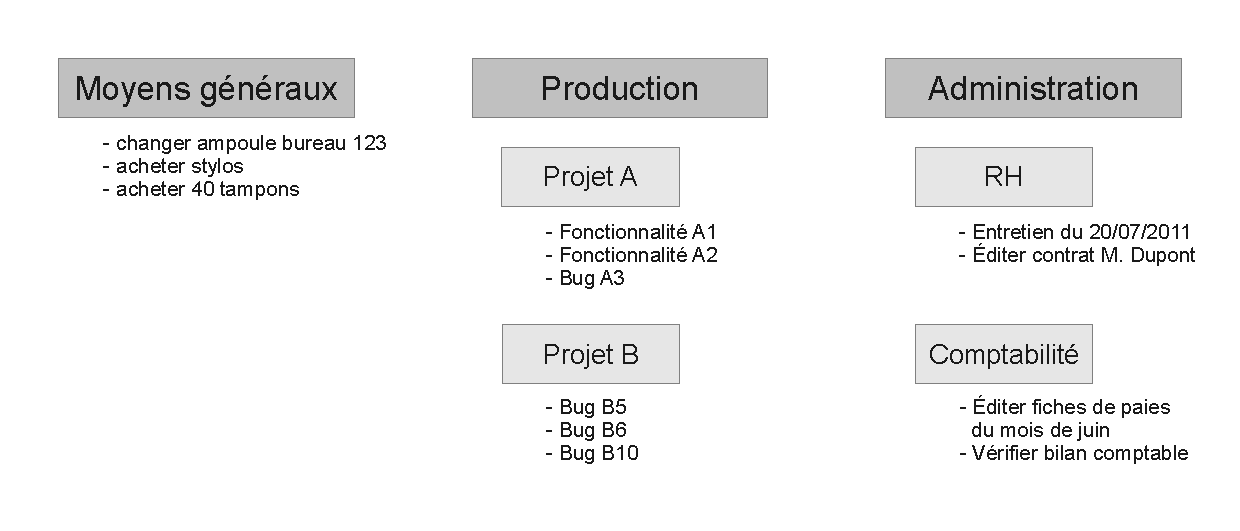
\includegraphics[width=13cm]{pic/taches}
	\caption{Exemple d'organisation d'un système de gestion de tâches pour une entreprise factice}
	\label{figure:pic-projet:taches}
\end{figure}

\paragraph{}
Un exemple de découpage des besoins d'une entreprise est représenté en \reffigure{pic-projet:taches}.

\paragraph{}
Finalement, ce type d'outil est complètement adapté à la gestion de projet agile.
Toutes les fonctionnalités qu'il intègre permettent une communication efficace de l'avancement du projet entre tous ses acteurs.
Aussi, sa facilité d'utilisation et les notifications des changements permettent d'accéder à une flexibilité maîtrisée.



\subsection{Outils}

\subsubsection{Redmine}

\paragraph{}
C'est le principal outil open source proposé par \asmile{} à ses clients.
Développé en Ruby avec le framework \aror, il a le gros avantage d'avoir une communauté très active.
Il s'utilise via le navigateur web.
Redmine est doté d'un bon nombre de fonctionnalités citées précédemment, parmi lesquelles :

\begin{itemize}
	\item une gestion en projets et sous-projets ;
	\item un système de gestion de tâches ;
	\item une vue des tâches sous la forme de GANTT ou de calendrier ;
	\item une gestion de feuilles de route\footnote{Dans le milieu informatique, ce terme est souvent utilisé (concurremment avec l'anglicisme \etranger{roadmap}) pour désigner le programme de développement d'un logiciel. Concrètement, on affecte les différentes tâches à réaliser à des jalons (ou versions). L'organisation et les priorités du développement apparaissent alors plus clairement.} ;
	\item un wiki\footnote{En informatique, un forum est un espace de discussion publique (ou au moins ouvert à plusieurs participants). Les discussions y sont archivées ce qui permet une communication asynchrone (c'est ce qui différencie les forums de la messagerie instantanée).~\cite{forum}} par projet ;
	\item un forum de discussion par projet ;
	\item un hébergement de fichiers et une gestion de documents par projet ;
	\item une intégration avec de nombreux systèmes de gestion de versions de code source (\cfsection{pic-source}) ;
	\item des notifications par e-mail ;
	\item une gestion fine des droits utilisateurs ;
	\item des groupes d'utilisateurs ;
	\item un support multilingue\ldots
\end{itemize}

De plus, Redmine est extensible par le biais de plugins.
Ainsi, de nombreuses fonctionnalités développées par la communauté peuvent être ajoutées, comme une gestion de budget ou une gestion de documents avancée par exemple.
Cela rend également possible le développement de fonctionnalités spécifiques pour répondre aux besoins pointus des clients.

Par ailleurs, \asmile{} propose également d'utiliser Redmine pour répondre à des besoins non-informatiques, comme évoqué précédemment.

\paragraph{}
Des captures d'écran de Redmine sont accessibles en \refannexe{redmine}.



\subsubsection{JIRA}

\paragraph{}
C'est un outil de gestion de projet similaire à Redmine du point de vue qu'il s'utilise par le biais d'une interface web.
Par contre, c'est un logiciel propriétaire développé en Java par Atlassian Software Systems.

Proposer un logiciel propriétaire n'est pas commun chez \asmile.
En fait il d'avère qu'il est complet et qu'il a beaucoup plu à Rexel, un des clients de \asmile{} qui a commandé l'intégration des autres outils open source de l'offre.

Son atout le plus notable est l'ensemble des représentations graphiques qu'il propose, mettant en relief les données des différents projets suivis.

\paragraph{}
Des captures d'écran de JIRA sont accessibles en \refannexe{jira}.



\subsection{Missions}

\subsubsection{Formation JIRA chez Rexel}

J'ai eu l'occasion de participer au début de mon stage à la formation JIRA donnée chez Rexel par mon maître de stage \agulet.
J'ai pu ainsi découvrir le produit, ses fonctionnalités et ses possibilités.



\subsubsection{Développement Redmine pour RAGT}

\paragraph{}
Pendant mon stage, \agulet{} a effectué une mission dans l'entreprise RAGT qui a commandé une mise en place complète de l'outil Redmine ainsi qu'une prestation de conseil.
Confronté à des problématiques spécifiques, il m'a demandé d'ajouter de nouvelles fonctionnalités au système de gestion de projets.

À cette occasion, j'ai appris à développer en langage Ruby et je me suis confronté à la documentation du framework \aror{} et à celle de Redmine.

\paragraph{}
Le premier développement a consisté à améliorer le système de gestion de tâches existant.
Dans Redmine, il est possible de lier des tâches entre elles en précisant le type de lien (\og lié à \fg, \og précède \fg, \og suit \fg, \og bloque \fg\ldots).
Ainsi, j'ai apporté la possibilité de créer à la volée une tâche à lier à une tâche existante.

\paragraph{}
Pour le second développement, j'ai amélioré un plugin existant : Better GANTT Chart.
Celui-ci améliore les graphes GANTT des tâches en ajoutant des flèches pour représenter les dépendances inter-tâches, issues des liens décrits précédemment.

Or, dans Redmine, il est possible de lier une tâche d'un projet à celle d'un autre projet.
Le problème est que les tâches issues d'un projet différent ne sont pas dessinées sur le GANTT. 
Je me suis alors chargé d'ajouter cette fonctionnalité que l'équipe à l'origine du plugin s'est empressée d'intégrer dans leur base de code.

\paragraph{}
Enfin, le dernier développement a concerné la possibilité de mettre en place des sous-groupes d'utilisateurs.
En effet, les groupes regroupent des utilisateurs de façon à les associer en masse à un projet donné.
Mettre en place des sous-groupes consiste à inclure des groupes dans un autre : de cette façon il est possible de construire une organisation complexe en évitant de répéter des affectations. 

Cette fois, j'ai développé directement dans le c\oe ur de Redmine et j'ai soumis la fonctionnalité à l'équipe qui dirige le développement.
Malheureusement, rien n'a pu être intégré pour l'instant faute de réponse.



\section{Gestion de versions du code source}
\label{section:pic-source}

\paragraph{}
La gestion de versions du code source est l'outil de prédilection d'une équipe de développement agile.
En effet, elle permet de suivre l'ensemble des modification effectuées sur le code de façon incrémentale.
Par ailleurs, il faut noter qu'elle ne se borne pas au versionnement de code source.
Il est ainsi possible de stocker dans un dépôt tout ficher texte, mais aussi tout fichier binaire (e.g. images, documents Office, etc.).

\paragraph{}
En pratique, à chaque fois qu'un fichier est ajouté au dépôt\footnote{Un dépôt est l'endroit virtuel où sont stockés les fichiers source.} ou qu'il est modifié, son état courant est sauvegardé de façon à pouvoir éventuellement être récupéré plus tard.
Ces versions gelées prennent le nom de \emph{révisions}.
Elles sont dotées d'un identifiant -- qui peut être un simple numéro ou bien un hash\footnote{On nomme fonction de hachage une fonction particulière qui, à partir d'une donnée fournie en entrée, calcule une empreinte servant à identifier rapidement, bien qu'incomplètement, la donnée initiale.~\cite{hash}} -- et contiennent un certain nombre d'informations utiles comme le nom et l'adresse e-mail de l'auteur, la date de création, un message descriptif des changements, etc.
En outre, on appelle \acommit{} l'action de créer une révision.

\paragraph{}
L'utilisation d'un système de gestion de versions apporte de nombreux avantages.
En effet, la pratique ancestrale consiste à copier l'ensemble du code source de l'application manuellement, soit à des points clés du cycle de développement -- comme les jalons par exemple -- soit de manière sporadique -- au bon vouloir des chefs de projet et des développeurs.
Pour le coup, une telle méthode est tout à fait inefficace du point de vue qu'elle est régulièrement soumise à des erreurs humaines, et qu'elle est abusivement consommatrice en espace de stockage alors que les différences entre les sauvegardes peuvent être très limitées.

Au contraire, la gestion de versions donne la possibilité d'automatiser de tels processus, permettant ainsi d'aider à tendre vers une industrialisation du développement logiciel.
Les deux inconvénients de la sauvegarde traditionnelle cités précédemment sont résolus, car le versionnement régulier est favorisé et car le stockage des révisions se fait de manière incrémentale, respectivement.

De plus, il devient possible de travailler de manière vraiment collaborative : plusieurs développeurs peuvent travailler sur les même fichiers source sans pour autant se gêner les uns les autres.
Dans le cas où une même portion de code est modifiée par plusieurs personnes, un conflit est détecté et doit être résolu manuellement : c'est une simple étape complètement intégrée au processus.

Un outil de gestion de versions facilite également la résolution de bugs, en permettant de naviguer aisément entre les différentes versions de fichiers source.
Étant donné que la granularité des changements entre deux révisions consécutives est relativement fine, on peut détecter l'instant précis où un bug a été introduit et éventuellement annuler les changements de la révision impliquée.

Enfin, la gestion de versions permet de réduire les appréhensions liées au développement de nouvelles fonctionnalités expérimentales.
Partir dans un nouveau développement indépendant alors que des changements doivent toujours être effectués sur une version dite stable -- celle en production par exemple -- ne pose plus problème.
Les outils donnent la possibilité de fusionner des bases de code qui ont évolué de façon distincte -- appelée \emph{branches} -- par le même système de gestion des conflits qui a été cité précédemment.

\paragraph{}
Versionner le code source de son logiciel n'apporte donc que des avantages.
La seule contrepartie réside dans le fait que les développeurs doivent être formés à l'outil choisi et motivés par son utilisation.
En effet, en tant que premiers utilisateurs du système, ils doivent en voir les bénéfices pour appliquer les bonnes pratiques inhérentes.

\paragraph{}
L'ensemble du jargon spécifique à la gestion de version qui a été évoqué dans cette section est illustré en \reffigure{pic-source:jargon-depot} et en \reffigure{pic-source:jargon-branches}.

\begin{figure}
	\centering
	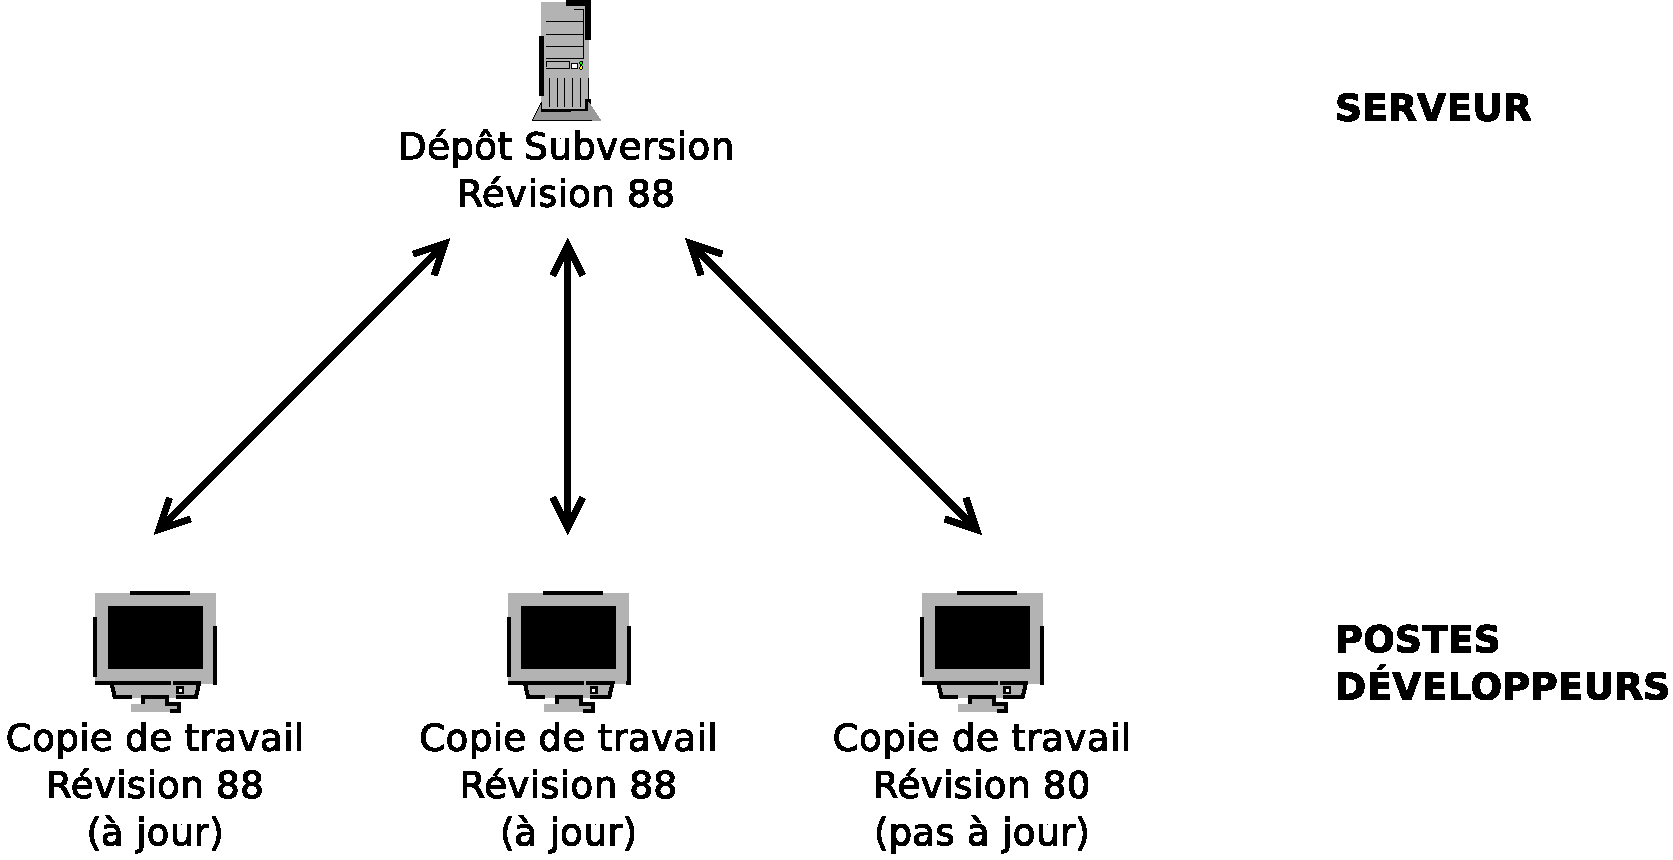
\includegraphics[width=12cm]{pic/jargon-depot}
	\caption{Illustration des concepts de dépôt et de copie de travail}
	\label{figure:pic-source:jargon-depot}
\end{figure}

\begin{figure}
	\centering
	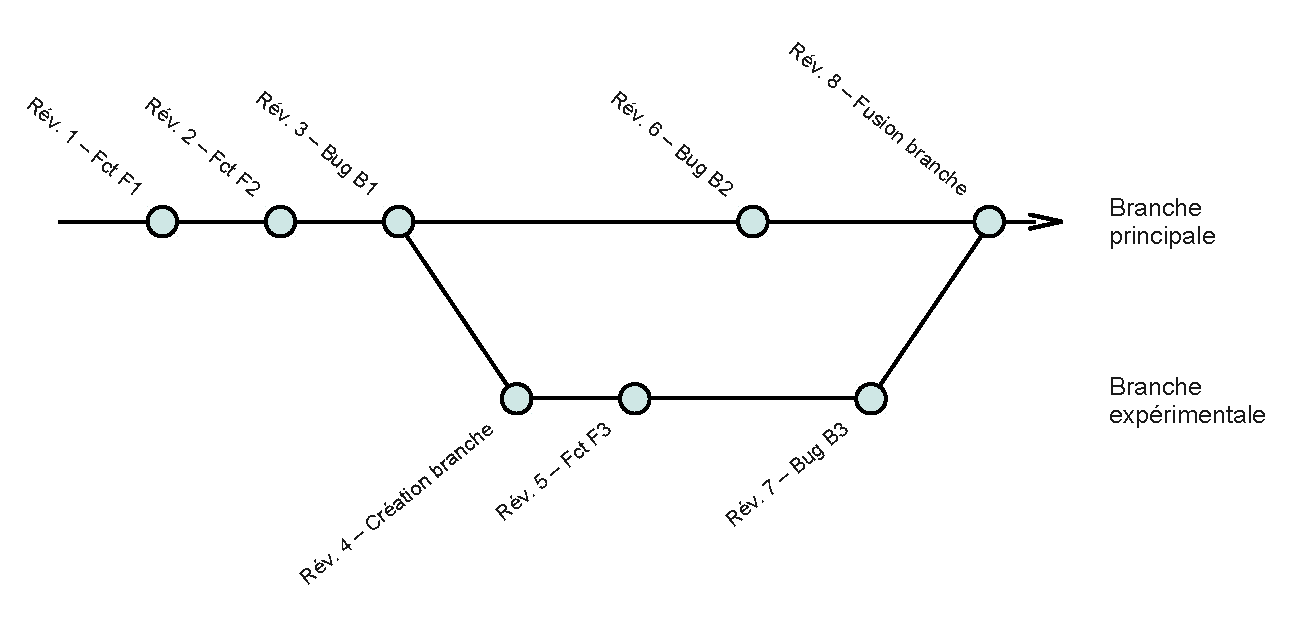
\includegraphics[width=14cm]{pic/jargon-branches}
	\caption{Illustration des concepts de révisions et de branches}
	\label{figure:pic-source:jargon-branches}
\end{figure}



\subsection{Outils}

\subsubsection{Subversion}

\paragraph{}
Subversion, souvent abrégé SVN, est certainement l'outil open source de gestion de versions le plus répandu dans les entreprises aujourd'hui.
Malgré l'apparition relativement récente de plusieurs solutions concurrentes, il reste encore massivement utilisé par les communautés open source pour gérer le code de leurs projets.


\paragraph{}
Il permet une gestion de versions dite \emph{centralisée}.
Cela implique qu'il n'existe qu'un seul dépôt de référence répertoriant l'ensemble des révisions.
Chaque développeur utilise un client Subversion afin de récupérer une \emph{copie de travail} locale du projet.
Il peut ensuite envoyer ses modifications des fichiers au dépôt sous la forme de révisions, à la seule condition que la copie de travail soit à jour.

Le modèle centralisé donne l'avantage d'être simple à appréhender, c'est le plus répandu dans le monde professionnel du fait de sa maturité.
Néanmoins, son inconvénient réside le fait que toutes les révisions soient stockées uniquement sur le dépôt.
Si ce dernier n'est plus accessible, les clients de l'outil ne sont pas capables d'être autonomes et ne peuvent plus remplir leurs fonctions.

À ce modèle on oppose la gestion de versions dite \emph{décentralisée} qui, elle, implique qu'il n'y ait pas de dépôt unique répertoriant l'ensemble de révisions.
En fait, chaque copie de travail est un dépôt à part entière contenant toutes révisions et que l'on synchronise régulièrement avec le dépôt considéré comme \og principal \fg.



\subsection{Missions}

\subsubsection{Formation Subversion chez Rexel}

Au même titre que la formation JIRA, j'ai également pu participer au début de mon stage à la formation Subversion donnée chez Rexel par \agulet.
Je connaissais déjà très bien l'outil, j'ai principalement appris de la façon de le présenter à un client.



\subsubsection{Proposition d'architecture Subversion pour Rexel}

Rexel possédait déjà un certain nombre de dépôts SVN dont l'architecture avait été mise en place par \asmile.
Externalisant la plupart du temps ses tâches de développement, le client souhaitait trouver une solution dans le cas où le prestataire de service désire travailler sur son propre dépôt SVN chez lui en interne.
Avec \agulet, nous avons fait plusieurs propositions de solutions :
\begin{itemize}
	\item utiliser un système de miroirs de dépôts -- Rexel posséderait alors un dépôt miroir en lecture seule de celui du prestataire ;
	\item le prestataire développe sur son propre dépôt, et à chaque livraison une révision est créée sur le dépôt de Rexel qui reste indépendant ;
	\item migrer vers un système de gestion de versions décentralisé.
\end{itemize}

Finalement, le client n'a pas donné suite à nos propositions et a conservé son système en l'état.



\section{Tests des applications}

\subsection{Tests unitaires}

\subsection{Tests fonctionnels}

\subsection{Outils}

\subsubsection{Selenium}

\subsection{Missions}

\subsubsection{Formation Selenium chez Spir}



\section{Intégration continue}

\paragraph{}
Le concept d'intégration continue consiste à tester automatiquement l'application tout au long de son développement.
Cela permet de prévenir les régressions et de détecter facilement où et quand des erreurs ont été introduites.

À l'échelle du développeur ou du chef de projet, lancer les tests d'un projet moyen doté une bonne couverture de tests prend beaucoup de temps.
C'est pour cela que les jeux de tests sont lancés de manière complètement automatique par un outil nommé \emph{plateforme d'intégration continue} (PIC).
Il est utilisé conjointement avec un système de gestion de version pour manipuler le code source.

\paragraph{}
En effet, pour chaque projet en cours de développement, la plateforme d'intégration continue surveille constamment si de nouveaux changements ont été introduits sur leur dépôt de code source respectif.
À intervalle de temps régulier, elle reconstruit chaque projet ayant fait l'objet de modifications depuis la passe précédente.
Les tests qui ont été écrits par les développeurs sont alors lancés.
À l'issue de la passe de tests, un rapport est sauvegardé.
Grâce au système de gestion de version, il est possible de savoir à quelle révision des bugs ou des régressions sont apparues.
 Enfin, l'état du projet -- en succès ou en échec -- est indiqué clairement aux visiteurs de la PIC.

Cet état peut être communiqué aux personnes intéressées de manière plus directe.
Il est par exemple possible de mettre en place des notifications par e-mail, messagerie instantanée, SMS voire même via les réseaux sociaux.

\paragraph{}
Avec l'intégration continue, on pousse au maximum les bénéfices des tests pour assurer la qualité logicielle du projet.
De plus, les PIC sont un outil idéal pour la mise en place de méthodes agiles.
En effet, lancer des tests de manière continue favorise la flexibilité en permettant de se lancer de façon réactive dans des changements plus ou moins importants.
La couverture de tests donne la possibilité de détecter les éventuelles régressions qui seront localisées dans le code et dans le temps grâce aux données des différents rapports issus de la PIC.



\subsection{Outils}

\subsubsection{Jenkins}

\paragraph{}
Jenkins est la PIC open source la plus populaire actuellement.
Écrite en Java, elle fonctionne dans un conteneur de servlets et est administrable via une interface web.

\paragraph{}
Chaque projet est listé sur la page principale de la PIC.
Un code couleur lui est associé : bleu en cas de succès de l'exécution du jeu de test, rouge en cas d'échec, jaune pour \og instable \fg{} et gris pour \og inconnu \fg.
La tendance récente de l'état du projet est même reportée via la métaphore de la météo : un icône représentant un soleil, des nuages ou un orage.

\paragraph{}
De base, la configuration du lancement des tests du projet s'effectue via de simples scripts shell UNIX ou batch Windows.
Pour les projets Java, il est également possible de reposer sur des scripts Ant\footnote{Ant est un projet open source de la fondation Apache écrit en Java qui vise le développement d'un logiciel d'automatisation des opérations répétitives tout au long du cycle de développement logiciel, à l'instar des logiciels Make. Ant est principalement utilisé pour automatiser la construction de projets en langage Java, mais il peut être utilisé pour tout autre type d'automatisation dans n'importe quel langage.~\cite{ant}} ou Maven\footnote{Maven est un outil open source pour la gestion et l'automatisation de production des projets logiciels Java en général et Java~EE en particulier. L'objectif recherché est comparable au système Make sous UNIX : produire un logiciel à partir de ses sources, en optimisant les tâches réalisées à cette fin et en garantissant le bon ordre de fabrication. Il est semblable à l'outil Ant, mais fournit des moyens de configuration plus simples, eux aussi basés sur le format XML. Maven est géré par l'organisation Apache Software Foundation.~\cite{maven}}.

L'exécution des tests peut être initié par différents moyens, comme des mécanismes de planification similaires au cron\footnote{cron est le nom d'un programme qui permet aux utilisateurs des systèmes UNIX d'exécuter automatiquement des scripts, des commandes ou des logiciels à une date et une heure spécifiées à l'avance, ou selon un cycle défini à l'avance.~\cite{cron}} ou une surveillance d'un dépôt de code source, entre autres.

En outre, il est possible de distribuer les le lancement des tests de chaque projet sur des machines différentes.
Les projets sont configurés sur un serveur Jenkins maître qui peut redistribuer ses tâches sur des serveurs esclaves mis en place sur d'autres machines.

\paragraph{}
Enfin, la force de Jenkins est son architecture modulaire.
Chaque fonctionnalité prend la forme d'un plugin qui peut être activé ou non de façon à ne pas alourdir ni l'interface de configuration ni le système.
Ainsi, aucune technologie n'est privilégiée avec Jenkins.
Seuls les plugins les plus importants sont fournis de base, alors qu'une communauté très active de développeurs propose régulièrement des plugins à la pointe des tendances actuelles.

On trouve notamment l'intégration avec Redmine, Subversion ou Selenium. 

\paragraph{}
À noter que Jenkins peut également être utilisé pour autre chose que l'exécution de tests.
Une autre utilisation concerne la construction ou la compilation\footnote{La compilation est l'action de traduire un langage (appelé le langage source) en un autre (le langage cible), généralement dans le but de créer un exécutable.~\cite{compilation}} régulière de projets de développement.

\paragraph{}
Des captures d'écran de Jenkins sont accessibles en \refannexe{jenkins}.



\subsection{Missions}

\subsubsection{Paramétrage de la PIC de Spir}

Pendant mon stage, j'ai eu l'occasion de mettre en place un projet pilote sur la PIC Jenkins de Spir.
Il concernait l'exécution de tests Selenium, étant donné que le client voulait s'équiper de cet outil.



\subsubsection{Formation Jenkins chez Spir}

La formation Selenium chez Spir évoquée précédemment a été suivie par une formation Jenkins décrivant l'intégration de tests Selenium dans la PIC.
C'est une formation que j'ai préparée en amont moi-même et que nous avons présenté au client en duo avec \agulet.



\section{Bilan}



